\chapter{Key-value databases}
\section{Redis}
\chapterauthor{Laura Khaze, Leon Sch\"urmann}

Redis is a key-value data store. It was invented by Salvatore Sanfilippo in
April 2009 and is released under the \gls{bsd} 3-clause (\textit{new} /
\textit{revised}) license. Therefore, it is a free and open source software
product. Redis -- originally an acronym for \textit{remote dictionary server} --
is primarily used as a database, caching-solution or a publish/subscribe message
broker.

Redis stands out in the field of key-value data stores because of its simplicity
and speed. A part of the high performance can be attributed to the use of
in-memory data structures, while the use of C -- a low-level systems programming
language -- provides some advantages as well. Because of its unique properties,
Redis is very popular. According to \texttt{db-engines.com}, it is currently on
rank seven of the most popular databases, and on rank one of all measured
key-value data stores \parencite{dbenginesRanking}.

The goal of this section is to show the primary characteristics and available
data types of Redis. Clustered Redis setups will be evaluated in the context of
the \gls{cap}. Finally, typical usage scenarios for this software will be
evaluated, and the most important facts are reiterated in the conclusion.

\subsection{Primary characteristics}
Redis has a few distinctive characteristics that make it unique in the set of
\gls{nosql} databases covered by this book. This section will evaluate these
characteristics in regards to the overall influence on the software.

\subsubsection*{In memory}
Redis is designed to run completely \textit{in-memory}
\parencite{redis:introduction}.  Traditional databases rely on their data being
stored on a hierarchical file system, typically on top of a mass storage medium
like \glspl{hdd} or \glspl{ssd}. While these media often come in
much larger sizes than \gls{ram} modules, and have a significantly less cost
per gigabyte, storing data on them has a few drawbacks.
For instance with \glspl{hdd}, accessing data at a specific position on the
disk requires waiting for a data seek operation to complete -- essentially
letting the physical platter spin to the sector where data is stored and moving
the read/write head into position. This makes random read and write operations
slow. Even with flash-based storage like \glspl{ssd}, where seeking data is not
an issue, there are many layers of abstraction between the virtual file system
and the physical data storage. Accessing a file on file systems typically
involves performing a so-called \textit{context switch} into the operating
system kernel, accessing a hardware controller, serializing data over a wire
according to standards like \acrshort{sata}, and the disk controller finally
accessing the data. All of these operations take a considerable amount of time.
\parencite{edgar}
However, when an application accesses its own main memory region in the system's
\gls{ram}, these operations get processed natively in the \gls{cpu} and
\gls{iommu} hardware, without involvement of the operating system kernel or any
peripherals.

In summary, storing data in \gls{ram} has advantages to system load, seek times,
response times and available bandwidth. However, at the time of writing,
\gls{ram} is significantly more expensive than traditional storage media. The
cost per gigabyte ratio could be higher then 238x (when comparing recent prices
of a $512GB$ \acrshort{ddr4} \acrshort{ecc} memory stick with a $4TB$ $7200rpm$
enterprise \gls{hdd}).

Because \gls{ram} is a form of volatile memory, after a power loss or system
reset, the data is cleared. To prevent data loss with Redis, two types of
persistence modes can be used \parencite{redis:persistence}:
\begin{itemize}
    \item \textbf{\texttt{RDB} files}:\\
	Redis can dump its entire data set into a binary \texttt{RDB} file that
        is sufficient to restore a full and consistent snapshot of a Redis instance.
        However, creating this dump takes time and memory -- Redis forks its primary
        process and therefore duplicates the entire in-memory data set. Copy-on-write
        techniques can reduce system load with this process. It is unfeasible to use
        this method for continuously storing the database's state.
        \parencite{redis:persistence}

    \item \textbf{\texttt{AOF} files}:\\
	Redis logs all of its transactions into an \texttt{AOF} file which can
        then be used to reconstruct a full snapshot of a Redis instance. This file has
        the advantage of being append-only, reducing random accesses and seek times. In
        addition to that, new transactions can be constantly written to this file
        without interrupting the primary Redis thread. However, as new transactions can
        make old ones irrelevant, these files are often not as compact as \texttt{RDB}
        database dumps. Therefore, they can be compacted to contain only required
        transactions to rebuild the current database state. \parencite{redis:persistence}
\end{itemize}

\subsubsection*{\acrshort{resp}: \acrlong{resp}}
To communicate with a Redis instance, a client has to use the \gls{resp}. The
primary goals of this protocol are to be simple to implement, fast to parse and
to be human readable. While it only relies on a bidirectional communication
channel with some guarantees regarding safety and packet order, it is currently
only implemented on top of \gls{tcp} or UNIX sockets. \parencite{redis:protocol}

\gls{resp} is designed to adhere to a request-response pattern. Both the
requests to the server instance, as well as the responses have a well-defined
human readable format. Different parts of the protocol are always terminated
with a carriage-return and new-line character (\texttt{CR LF} or
\texttt{\char`\\ r\char`\\ n}). \parencite{redis:protocol}

Each request is an array of a Redis command and additional string arguments. The
length of the array, as well as the size of all strings is sent as a prefix to
the respective element. This has the advantage of being both simple to construct,
and Redis being able to allocate a fixed size chunk of memory for each element.
Therefore, once the data is received, no post-processing is required.
\parencite{redis:protocol}

The response for a request always starts with an \acrshort{ascii}-byte
indicating the response data-type. For instance, this could be "\texttt{-}" for
a string error, or "\texttt{:}" for a string-encoded integer that is guaranteed
to be a valid $64$ bit signed integer value. Following this byte, the payload is
encoded as a (depending on the type \textit{binary safe}) string.
\parencite{redis:protocol}

Overall, the Redis protocol achieves its goals of speed, simplicity and human
readability. Its properties make it easy to develop libraries for communication
with Redis.

\subsection{Data Types} \label{redis:dataTypes}
Redis is not only a key-value data store but rather a data structures server. In a
classical key-value data store a string value is accessed via a string key while
Redis supports several other data structures (hashes, sorted sets, etc.). The
basic data structures as well as some extraordinary ones will briefly be
described in this section. \parencite{redis:dataTypesIntroduction}

\subsubsection*{Strings}
Strings are the most basic data type used in a Redis data store on which all
complex data structures are built. Strings are binary safe, which means it is
possible to save any kind of data (max 512MB per key), like a \gls{jpeg}
image or a serialized Ruby object, as well as simple text.

Moreover, it is possible to use strings as atomic counters using commands in the
\texttt{INCR} familiy (\texttt{INCR}, \texttt{INCRBY}, etc.). Since it is not
possible to declare an integer in Redis, strings are used for those purposes.
Furthermore, it is possible to use strings as random access vectors due to
commands like \texttt{GETRANGE}, \texttt{SETRANGE} or \texttt{GETBIT}.
\parencite{redis:dataTypesIntroduction, redis:commands, redis:dataTypes}

\subsubsection*{Lists}
Redis lists are a collection of strings sorted by insertion order with a maximum
length of $2^{32}-1$ strings. Among other operations, it is possible to insert
and delete elements within a list (either from the head or tail), as well as
getting a subset of a list. A list is created when a push operation is
performed on an empty key and conversely a list is deleted (key clearance) if
the list is emptied by an operation.

Due to the combination of some operations, it is possible to create a customized
list for specific use cases. For instance, it is possible to use \texttt{LPUSH}
and \texttt{LTRIM} to create a list with a defined length which will never
exceed a certain number of elements.  Moreover lists can be used to model a
timeline in a social network like Instagram or Facebook. In this example it
would be possible to add new elements in the time line (\texttt{LPUSH}) and
receive only the most recent events (\texttt{LRANGE}).
\parencite{redis:dataTypesIntroduction, redis:commands, redis:dataTypes}

\subsubsection*{Sets}
Unlike lists, sets are an \textit{unordered} collection of strings with a
maximum number of $2^{32}-1$ elements.
Elements within a set are called members. Members can be added, removed and
returned from a set (\texttt{SADD}, \texttt{SREM}, \texttt{SPOP}). If a string
is already contained within the set, it is not possible to add it again. In this
case, Redis will simply not add the member, without indication of an error.
Thus, it is not necessary for an application to use \texttt{SISMEMBER} before
calling the \texttt{SADD} operation on a set. Moreover it is possible to display
all members of a set and check whether a specific member is contained within a
set (\texttt{SMEMBER}, \texttt{SISMEMBER}).

Due to the characteristics of the \texttt{SADD} function, sets can be used to
track unique things like students ids lending a specific book in the library.
\parencite{redis:dataTypesIntroduction, redis:commands, redis:dataTypes}

\subsubsection*{Hashes}
Hashes are the most suitable data type to represent objects, since they are maps
between string fields and string values. Every hash can store up to
$2^{32}-1$ field value pairs.

It is possible to set fields and retrieve the value of fields, both either
individually or simultaneously (\texttt{HSET}, \texttt{HMSET}, \texttt{HGET},
\texttt{HMGET}). \parencite{redis:dataTypesIntroduction, redis:commands,
redis:dataTypes}

\subsubsection*{Sorted Sets}
Similar to sets, sorted sets are non repeating collections of strings ordered by
a non-unique score (smallest to greatest).  Members within a sorted set can be
added, removed and returned (\texttt{ZADD}, \texttt{ZPOPMIN}, \texttt{ZPOPMAX}).
Moreover it is possible to return members with a certain score or at a certain
position/index within the sorted set. Also, scores can be increased and thereby
updated.

Thus sorted sets can be used to keep track of any kind of ranking like a
competition. In this case, scores can be initially inserted and later updated using
\texttt{ZADD}.  Due to operations like \texttt{ZRANGE} or \texttt{ZRANK}, it is
possible to receive the top or bottom half of the ranking, or receive the rank
of a specific member. \parencite{redis:dataTypesIntroduction, redis:commands,
redis:dataTypes}

\subsection{Multi-node setups / Redis Cluster} \label{redis:multiNodeSetup}
Originally, Redis only supported single-node and non-clustered setups. In
combination with its mostly single-threaded architecture, this allowed it only
scale vertically.  However, with the introduction of both external clustering
mechanisms (where a so-called proxy would distribute and balance requests across
different Redis instances) and internal clustering support, Redis can now scale
horizontally as well. Because of the variety of clustering solutions, and focus
on Redis itself, external proxies are out of the scope of this evaluation.

The integrated clustering solution of Redis is called \textit{Redis Cluster}.
According to its documentation, \textit{"[it] is a distributed implementation
of Redis"} \parencite{redis:clusterSpecification} and has three primary goals:

\begin{itemize}
    \item \textbf{High performance and linear scalability} up to 1000 nodes
    \item \textbf{Write safety}
    \item \textbf{Availability}
\end{itemize}
However, by specification, these criteria do not have to be guaranteed at all
times -- altogether or even on their own. \parencite{redis:clusterSpecification}

Nodes in a Redis Cluster setup are connected over \gls{tcp} bus connections.
These connections (bus) are used to propagate information to all nodes in the
cluster. Client requests to nodes in the cluster are not forwarded to the
data-holding node. Instead, the client is redirected to the correct node by the
use of \texttt{MOVED} or \texttt{ASK} error return codes.
The data distribution is decided by the CRC-16 value of the string key. Each
unique CRC-16 value is called a keyslot. All keyslots have one master and
$n \geq 0$ slave nodes.
\parencite{redis:clusterSpecification}

\subsubsection*{Positioning in the CAP theorem}
In the following, different criteria of Redis Cluster regarding typical usage
guarantees in a distributed setup are evaluated:
\begin{description}
    \item \textbf{Consistency}:\\
        According to the official Redis website, \textit{"Redis is not able to
        guarantee strong consistency"} \parencite{redis:clusterTutorial}. This can be implied
        from a few scenarios.

        For instance, when a client writes a key to the respective master node
        for this keyslot, the operation is acknowledged instantly. The master then
        replicates this write to all slave-nodes for this keyslot. However, when these
        slave nodes are not reachable, the write is not fully synchronized across the
        network. In the case of a network partition, a slave that has not yet received
        this write operation may be promoted to become a master. The write is then lost,
        although it has been acknowledged. \parencite{redis:clusterTutorial}

	In another example, the network is partitioned into a master-majority and
        a master-minority partition. For a short amount of time, both partitions accept
        write operations which are also acknowledged. However, the minority-partition
        will eventually completely block any write operations. After the network is
        reunited, the previous writes to the minority-partition are simply discarded.
        Redis avoids merge operations, as these provide architectural challenges and
        might not work well on large data \parencite{redis:clusterSpecification}.
        \cite{redis:clusterTutorial}

    \item \textbf{Availability}:\\
	As already stated regarding the consistency of Redis Cluster, the
        minority-side of a network partition will refuse write-operations after a
        timeout. Therefore, Redis Cluster is not available.
        \parencite{redis:clusterSpecification}

	Even on the majority-side of the network, some write operations might be
        refused for a short amount of time. After an initial detection of a network
        partition and a timeout, slaves of missing keyslots get promoted to be master
        nodes. As soon as a master exists for all keyslots, the majority-partition is
        available again. \parencite{redis:clusterSpecification}
\end{description}

Depending on the kind of setup and test scenario Redis \textit{tends} to be
either AP or CP. Since this is only a small propensity, for systems or applications
requiring the characteristic AP or CP, a database designed for a clustering
solution should be used. This opinion is, in addition to the official documentation,
shared by \cite{redis:davis2015} and others.
Redis was initially designed as a single node solution with the primary focus on
performance.

\subsection{Typical use cases}
Redis can be used for a variety of different purposes and use cases. In the
following, three typical use cases are stated.

Redis can be used as a general purpose data store, especially if the data and
application requires simple data structures and high performance.  Nevertheless,
Redis is not suitable for every use case requiring a general purpose data store.
Since there are no complex data types, besides the ones mentioned in section
\ref{redis:dataTypes}, and it is not possible to model relations between
different data objects (as in a relational database), use cases with these
requirements can not be implemented using Redis. Moreover, the high memory usage
of Redis can either exceed the capacity of preexisting infrastructure, or
increase the cost of purchasing infrastructure drastically.

Due to these characteristics, Redis is often used to store volatile data, as a
caching mechanism or as a message broker. \parencite{redis:commands, redis:introduction}

\subsubsection{Caching}
Based on the characteristics of Redis, Redis is ideal for a caching mechanism.
Common \glspl{dbms} usually have high latencies and response times which could
make the user interface of an application feel sluggish.

\begin{figure}[h]
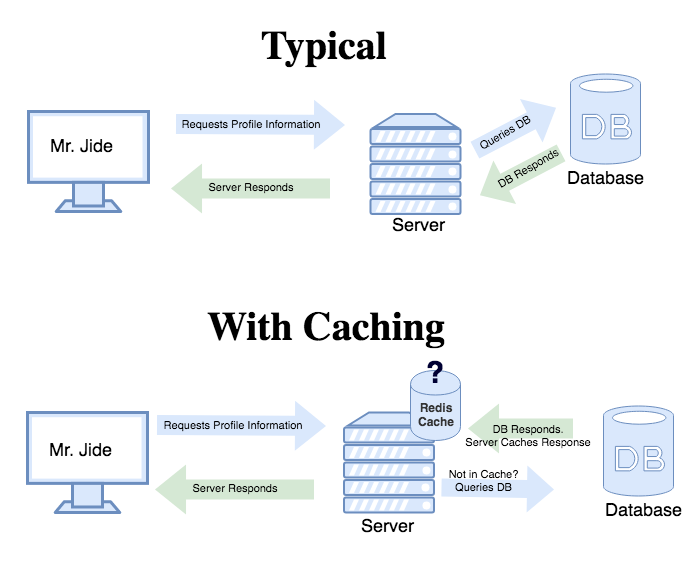
\includegraphics[width=12cm]{img/redis_caching.png}
\centering
\caption{Redis Caching Solution \parencite{redis:img:1}}
\label{fig:redisCaching}
\end{figure}

To solve this issue, a caching mechanism can be used. Already prepared and
computed data, which is used several times, is stored in the caching mechanism
with the result of less interaction between the user interface and the
\gls{dbms}.

In \textit{figure \ref{fig:redisCaching}}, the difference between server queries
to a database with and without Redis as a caching solution is pictured. The
second option (with a Redis cache) reduces the response time since only queries,
whose data is not already cached, are forwarded to the \gls{dbms}.

Redis-keys can be marked for deletion after a specified timeout (\texttt{TTL}),
and display the time that has elapsed since the key was last modified
(\texttt{OBJECT IDLETIME}). This enables automatic deletion of seldom used
data.  Thus Redis can be used as a caching solution for image previews, fetched
data from \acrshort{api}s, as well as session data. \parencite{redis:commands}

\subsubsection{Message broker functionalities}
Since Redis implements a publish-subscribe pattern, it is possible to use Redis
as a message broker.

A publish-subscribe pattern is a mechanism where subscribers can receive
information/messages from publishers. A typical publish-subscribe system
consists of several subscribers and several publishers, where one application can
be both subscriber and publisher. Publishers can provide information on specific
issues without any knowledge of possible subscribers. Each message is assigned
to a topic, which subscribers can subscribe to. In turn, these do not know if and
which publisher published on a specific topic. \parencite{redis:ibmPubSub}

Redis offers the typical publish-subscribe pattern features. Clients can
subscribe (\texttt{SUBSCRIBE}, \texttt{UNSUBSCRIBE}) to a topic as well as push
messages to a specific topic/channel (\texttt{PUBLISH}). The payload of the
message is a binary-safe string, which enables the clients to exchange any kind
of data.

This message broker functionality is especially useful for event notifications.
For instance the clients can be notified about changes within the data store.
Moreover, Redis' publish-subscribe implementation can be used to exchange
arbitrary data. However, because this is essentially a routed protocol, it is
less performant compared to peer to peer connections such as \gls{tcp} or UNIX
sockets. \parencite{redis:PubSub}

\subsection{Conclusion}
In this section, the key-value data store Redis was introduced by explaining the
main characteristics and some of Redis' data types. In addition to that, a
clustered Redis setup is analyzed in regards to characteristics from the CAP
theorem.  Finally, some of the most popular use cases were reiterated.

To summarize, Redis is much more than a traditional key-value data store.
Different data types, carefully chosen architectural decisions and a
speed-optimized implementation make it flexible and better suited for some
applications. For instance, Redis is an excellent data store for caching
purposes. While the publish- / subscribe feature does not necessarily have a
great influence on the storage features, it can be used in combination with
those to signal other Redis clients that some keys changed.

However, having a purely in-memory data store means that it is expensive to
operate with vast amounts of data. Also, data persistence is possible, but only
with a few disadvantages. Last but not least, Redis can be used in a clustered
setup. The internal clustering mechanisms (Redis Cluster) do not provide strong
guarantees regarding availability as well as consistency. This severely limits
its use-cases to applications, where both the correctness and presence of
distributed data is not a strict requirement.
